\chapter{Baseline Approach}

\section{Preprocessing}

Before starting to build a \acrshort{nlp} model it's mostly inevitable to preprocess the data you want your model to rely on. In many
\acrlong{ml} projects preprocessing is the most important part. A solid data basis can increase the performance of the model. Further
more it's very likely that preprocessed data is much more comfortable to deal with than raw data.

\subsection{Collecting Data}

As mentioned in \ref{chap:data-source} the source data is stored in two separate \acrshort{pst} files. To extract information out of this
proprietary file format a library called \emph{pypff}\footnote{Available at \url{https://github.com/libyal/libpff/wiki/Python-development}}
is used. The email messages are stored in different directories which either can have multiple sub-folders inside. Because of this structure
a recursive approach fits best to collect the data. Listing \ref{code:traverse} shows the detailed implementation including the calls to
parse (:13) and clean (:15) the message at the same iteration. The parser consists of three independent routines to get the message string
from HTML, RTF, and plain text emails. The cleansing procedure is explained in the next section.

\subsection{Data Cleansing}
\label{chap:cleansing}
As seen in section \ref{chap:typical-contents} there is a huge part of messages which shouldn't be used for further processing. This messages
should be cleared from the message pool. This discipline is called \emph{data cleansing} and can save a lot of time later on the project if
it's done carefully. But not all messages need to be removed completely from the data set. There exist a few cases where it's possible to only
remove certain pieces of a message like signatures or the forwarded parts which are added by default if you reply to an e-mail.

Listing \ref{code:regular-expressions} shows a sample of the used regular expressions to detect unwanted content within the messages. If a
junk pattern (:1-3) matches, the whole message is deleted. The forwarded parts of messages, which are often displayed as citations, are stripped
off with several patterns (:5-10). The regular expressions are made out of observations during the exploration of the data sources.

\begin{lstlisting}[language=Python, label={code:regular-expressions}, caption=Regular expressions for junk detection]
JUNK_1 = re.compile('^Fehler bei der Nachrichtenzustellung')
JUNK_2 = re.compile('^Submitted on(.)*Submitted values are:')
JUNK_3 = re.compile('^Form Returned: Telefonnotiz')

FORW_1 = re.compile(r"[-]{5}\s*(Message d'origine)\s*[-]{5}")
FORW_2 = re.compile(r'[-]{5}\s*Weitergeleitete Nachricht\s*[-]{5}')
FORW_3 = re.compile(r'Am \d{2}.\d{2}.(20)?\d{2} (um )?\d{2}:\d{2}')
FORW_4 = re.compile('Von:(.)*An:|From:(.)*To:')
FORW_5 = re.compile('Submitted on(.)*Submitted values are:')
FORW_6 = re.compile('GB Digitaler Kundensupport <(.)*> schrieb am')
\end{lstlisting}

Further showed the exploration that messages with a length of more than 3000 characters\footnote{The remaining length after stripping off signatures
and forwarded parts} are principally newsletters or spam. On the other hand messages with a remaining length of less than 75 characters aren't of
interest as well. Therefore only messages between these two boundaries are chosen for further processing steps.

The email messages are written mostly in German but you can find some other languages like French, Italian, and English in the raw data. The final
model should be able to predict named entities in German but not in foreign languages which would require a lot more training data and knowledge about
these languages. A data scientist at Swiss Mobiliar recently developed a library which combines four language recognition methods to predict the
language of a given text by simply calling all four functions and returning the language with the most votes. This library got the appropriate name
\emph{LangVoter} and is used to filter out any non-German messages.

After data cleansing the number of messages is sharply below the original amount. More than 55 percent of messages have been cleaned (see Figure
\ref{fig:plot-comparison-cleansing}). Figure \ref{fig:plot-comparison-cleansing-types} shows that the remaining data set consists of 10830 HTML
(-48\%), 949 plain text (-83\%), and 378 RTF messages (-60\%). As mentioned in section \ref{chap:data-source} many auto-generated messages are of
type RTF and plain text. Therefore it isn't surprising at all that most plain text and the bigger part of RTF messages don't contain valuable
information for the training of a \acrlong{ner}.

A reliable deep learning model should be trained with as many samples as possible to give reasonable predictions. With a total amount of 12157
messages and the right techniques to virtually increase the training set size, this might be enough for the beginning.

\begin{figure}[!ht]
    \begin{subfigure}{0.5\textwidth}
        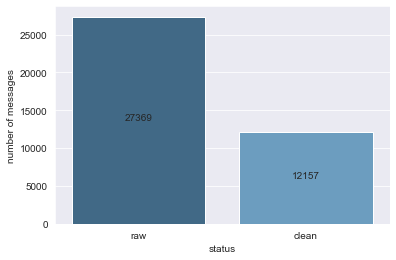
\includegraphics[scale=0.4]{plot-comparison-cleansing-total}
        \caption{Comparison in general}
        \label{fig:plot-comparison-cleansing}
    \end{subfigure}
    \begin{subfigure}{0.5\textwidth}
        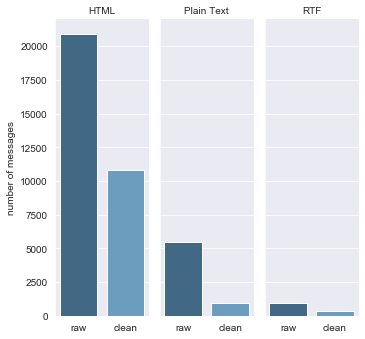
\includegraphics[scale=0.4]{plot-comparison-cleansing-type}
        \caption{Comparison grouped by type}
        \label{fig:plot-comparison-cleansing-types}
    \end{subfigure}
    \caption{Comparison before and after data cleansing}
\end{figure}


\subsection{Data Labelling}

In supervised learning a model needs to know the correct classification of the samples to compare them against its own predictions. The data set
is called pre-labelled. An inevitable part of a data scientist's work is to label data manually. Doccano\footnote{available at
\url{https://doccano.herokuapp.com}} is an open-source text annotation tool built for creating labelled data. It supports sequence to sequence
labelling which is useful for \acrlong{ner}.

\subsubsection{Doccano Parser}

One downside of Doccano are the limited options for exporting labelled data. You can download data only as JSON file with text labels. The exported
file has the same structure as listing \ref{code:doccano-export}. If the exported data should be used as validation set it needs to become more
handy to work with. Therefore I created a python library called \emph{mobi\_docparser}. The library allows users to parse Doccano's offset notation
into a list with two elements: The text after a simple whitespace tokenisation and the corresponding labels for each token, either in \acrshort{iob}
or binary notation. After parsing, the named-entity \emph{vodka martini} would be splitted into the tokens \emph{vodka} (B-DRINK) and \emph{martini}
(I-DRINK).

\begin{lstlisting}[label={code:doccano-export}, caption=Sample export from Doccano as JSON (text labels)]
{
  "id": 12162,
  "text": "Bond drinks his vodka martini shaken, not stirred.",
  "meta": {},
  "annotation_approver": null,
  "labels": [[0, 4, "per"], [16, 29, "drink"]]
}
\end{lstlisting}

\section{SpaCy Model}

SpaCy is meant to be the fast and easy-to-use \acrshort{nlp} library for the industry. Unlike more scientific libraries like NLTK\footnote{For more
information consider \url{https://www.nltk.org}}, spaCy focuses on getting work done rather than optimizing parameters to achieve even better results.
It's shipped with support for more than 53 languages including \acrlong{ner}, pretrained word vectors, and a non-destructive tokenization\footnote{
SpaCy's tokenization is fully reversible to reconstruct the original text} \cite{spacy}.

\subsection{Implementation}

Like the developers of spaCy mentioned on their homepage, it's very easy to integrate spaCy into your project. With just a few lines of code a pretrained
language model can process input texts.

\begin{lstlisting}[language=Python, label={code:spacy-integration}, caption=Sample of a runnable spaCy model]
import spacy

# load the German language model
nlp = spacy.load('de_core_news_md')

# process text
doc = nlp('Bond drinks his vodka martini shaken, not stirred.')

for token in doc:
    # print named-entities
    print(token.ent_type_)
\end{lstlisting}

There exist three German language models which can be used to process text. As seen in listing \ref{code:spacy-integration} (line 4) the medium-sized
news model is being used for this baseline approach. The model has a size of 214 MB and is able to recognise \emph{LOC}, \emph{MISC}, \emph{ORG}, and
\emph{PER} entities \cite{gh-spacy}. It's trained with data sources from the \emph{TIGER Corpus} and \emph{WikiNER}. The former has been trained with
approximately 50 000 sentences from the \emph{Frankfurter Rundschau} newspaper \cite{tiger}.

The \emph{WikiNER} corpus represents 7200 manually-labelled Wikipedia articles including the nine largest Wikipedias including English, German, Spanish,
and French. Unlike the \emph{TIGER Corpus}, the data quality of \emph{WikiNER} is only silver-standard. This means that the data is automatically created
by exploiting Wikipedia. Every link inside an article is getting replaced by the manually-labelled \acrshort{ne} category of the linked article \cite{Nothman}.

\subsection{Validation}

To validate spaCy's predictions the results need to be compared against the labelled \gls{mobi24} data. Because of the more sophisticated tokenisation
process of spaCy, the tokens aren't comparable with the output of the \emph{mobi\_docparser} library. Therefore spaCy's default tokenizer needs to be
overwritten with a simple whitespace tokenizer. As seen in listing \ref{code:tokenizer} the custom tokenizer simply uses the \verb|split()| function of
python's string module \cite{spacy-tok}.

\subsection{Performance}

Due to the fact that the model is trained on the \emph{TIGER} and \emph{WikiNER} corpus, it isn't very surprising that spaCy has it's difficulties with
recognising addresses because the corpora don't provide that many. SpaCy gets a mediocre \emph{f1 score} of \textbf{0.485}\footnote{Measured with the
current state of the labelling process (967 messages)}. As discussed in section \ref{chap:accuracy} the high accuracy of \textbf{0.946} shouldn't be used
as a performance indicator. The number of outside tokens compared to named entities is way to imbalanced. For more information refer to table \ref{tbl:perf-spacy}.
If both entity types are considered separately, there is a huge gap between the \acrshort{kpi}s. As seen in tables \ref{tbl:perf-spacy-per} and
\ref{tbl:perf-spacy-loc}, recognising only names has a more than eight times higher \emph{f1 score} than address recognition.

If we have a closer look at the predictions spaCy did, we can see that many domain specific language is misinterpreted. Considering table
\ref{tbl:spacy-wrong-predictions}, domain language like \emph{\Gls{Protekta}} or \emph{Mobiliar} are recognised as named-entities of type \emph{PER}. Even
very common words like \emph{Hallo}, \emph{Lieber}, and \emph{Gruss} are false predicted. These kind of words occur often before names, which might be
a possible reason why spaCy has its problems with.

\begin{table}[h!]
    \centering
    \begin{tabular}{|C{6em}|L{25em}|}
        \hline
        \textbf{Prediction} & \textbf{Exampe Tokens} \\ [0.5ex]
        \hline
        PER & Protekta, Mobiliar, Initial-Passwort, Weihnachtstage, Telefongespräch, Hauptstrasse, Hallo, Lieber, Gruss, Danke \\ [0.5ex]
        \hline
        LOC & Kundenportal, Mobirama, Gebäudeversicherung, Webbrowser, www.mobiliar.ch/login, Sicherheitsgründen, Datenschutzgründen, Mobiltelefon \\ [1ex]
        \hline
    \end{tabular}
    \caption{Examples of false spaCy predictions}
    \label{tbl:spacy-wrong-predictions}
\end{table}

It's very irritating that spaCy predicts URLs as addresses. These tokens follow a specific pattern and could be easily recognised by a simple
regular expression. Unlike false predicted names, the most common mispredictions for addresses cannot be grouped together that easily. The tokens are
often insurance related, but they seem to be distributed randomly.

\subsection{Conclusion}

SpaCy keeps what it promises. It's the easy-to-use library for processing texts. Within less than ten lines of code a fully working \acrlong{ner} can
be used to understand natural language. SpaCy's performance depends on the underlying model. According to the official website the medium-sized German
model should achieve an overall \emph{f-score} of more than \textbf{0.834} \cite{spacy}. This score nearly doubles the score spaCy achieved while
processing the \gls{mobi24} data.

The library offers to do a retraining with an individual labelled corpus. This would make the model familiar with the insurance context. It's uncertain
how much the performance would improve. Due to limited time resources the spaCy approach isn't developed further. But the spaCy model can be used as a
solid baseline model.

\section{Regex Model}
\label{chap:regex-model}
A written language consists of a word set and a rules set to describe how single words can be combined together to form larger constructs
like sentences or even texts. Every language follows a specific pattern which changes a lot over time. In information technology, there exist
regular expressions\footnote{Patterns for defining character sequences used for search, replace or validation operations} which are very useful
to locate such patterns inside text.

A basic implementation of a regular expression based algorithm for \acrlong{ner} may sound very costly if you have to define every language rule
as a regular expression. But it can be simplified by the use of reference data. These kinds of data are called dictionaries and let you lookup
certain words to classify them according to the dictionary they are part of. This seems to be a very solid basis for classifying text. But because
of word ambiguity it's very important to define how to proceed if a term occurs in multiple dictionaries and not to rely simply on them.

\subsection{Basic Dictionary Lookup}

This baseline approach starts with a simple dictionary lookup. Data scientists at Swiss Mobiliar created two dictionaries containing first and last names.
These lists are filled with a large amount of names due to different varieties of a single name and the different cultures people come from nowadays.
Together there are more than 140.000 names present.

\begin{lstlisting}[language=Python, label={code:regex-dict-lookup}, caption=Simple dictionary lookup]
import pandas as pd

first_names = pd.read_csv('./dictionaries/firstnames.csv', header=None, encoding='cp1252')[0]

def predict(token):
    if token in first_names:
        return 'PER'
    return 'O'
\end{lstlisting}

As seen in listing \ref{code:regex-dict-lookup}, the \emph{pandas} package is used to easily load data from the dictionary with a given encoding. \emph{CP-1252}
is an 8-bit encoding originally created for Microsoft Windows. Both name dictionaries are encoded with \emph{CP-1252}, sometimes also called \emph{ANSI}.

The dictionaries for addresses are manually created with data from the \emph{Federal Statistical Office} \cite{bfs}. There is a dictionary containing
all valid zip codes for Switzerland and another one with every municipality. Municipalities are stored in lowercase with escaped umlauts. This format
can be easily reproduced with just a few lines of python code. Another dictionary with a vast amount of street names is provided by another data scientist
at Swiss Mobiliar.

Table \ref{tbl:perf-regex} shows that the simple dictionary lookup approach only reaches an unpleasant precision of about \textbf{0.146}. Even though the very
decent recall of \textbf{0.733}, the resulting \emph{f1-score} is \textbf{0.243}. The lookup model's precision is much lower compared to the German spaCy model,
which means that there exist many tokens which are falsely predicted as named-entities. An enhancement to the current model should focus on increasing its precision.

\subsection{Enhancements}

Some improvements need to be made to increase the \emph{f1-score} of the baseline model. Table \ref{tbl:perf-spacy} refers to the resulting performance indicators. 

\subsubsection{Clean last names dictionary}

A detailed investigation shows that the last names dictionary contains many ambiguous values which are proper last names but have a different meaning in most scenarios.
The precision rises to a value nearly four times the original value if the last name lookup is being removed. Though the recall drops from \textbf{0.73} to \textbf{0.4}
because last names aren't recognised any longer. The optimal solution lies somewhere in between where many ambiguous values should be removed from the dictionary. But
this cleanup process will always reduce the recall.

\begin{quote}
    "Herren, Weiss, Guten, Franken, Grund, Juli, Mobiliar, Mobi, Kunde"
\end{quote}

After removing ambiguous values the precision jumps from originally \textbf{0.146} to \textbf{0.432} with a minimal loss on recall of only \textbf{1\%}. There are
several terms which are obviously not names like \emph{Mobiliar}, \emph{Mobi}, or \emph{Kunde} which are removed too.

\subsubsection{Add a scoring scheme}

A match in the dictionary might not be enough to determine the token's entity type. Therefore a scoring system can be helpful to given each feature an individual score.
Names and addresses are normally starting with an uppercase letter. With these two conditions the model's precision heightens to \textbf{0.487} with an unchanging
recall. 

\subsubsection{Compare against multiple variants}

Tokens might be all caps or without escaped umlauts or \gls{diacritic}s. It can be useful to lookup for several slightly modified versions of the original token. As
seen in table \ref{tbl:perf-regex} (rows 5/6), this enhancement lifts the \emph{f1-score} over \textbf{60\%}.

\begin{lstlisting}[language=Python, label={code:regex-variants}, caption=Creating different variants of a single token]
def create_variants(token):
    """
    Creates multiple variants of the same token for dictionary lookup
    """
    original = token
    cleaned = clean_token(token)
    small = umlauts.lower()
    umlauts = escape_umlauts(original)
    special = re.sub(r'[.,;:\-_]', '', small)
    diacritics = escape_diacritics(small)

    return {original, cleaned, small, umlauts, special, diacritics}
\end{lstlisting}

The newly created set of tokens can easily be compared with the dictionaries by using the \verb|intersection(t)| operation of the standard library.

\subsubsection{Involve the token's neighbours}

A valid address consists of several parts including the street name, street number, postal code, and municipality. Therefore these parts appear in a certain
sequence. After detecting a postal code in the previous processing loop there seems to be a significantly higher chance that a municipality will follow next.

Unfortunately there is no difference in recognising addresses. The \emph{f1-score} gains only \textbf{0.1\%} but the number of dictionary lookups nearly triples.
A possible reason might be, that there aren't that many addresses in the training and validation set. Due to this microscopic performance benefit and the extended
processing time, the changes are discarded.

\subsubsection{Naming dictionary clean up}

There are still many ambiguous tokens which are falsely predicted as names. After a more rigorous clean up of both naming dictionaries, the \emph{precision} climbs
from former \textbf{50.4\%} to pleasant \textbf{77.3\%}. This is done with a German stop words dictionary\footnote{Found online at
https://countwordsfree.com/stopwords/german} which values are intersected with the naming dictionaries. Every match is directly removed from the naming dictionaries.
Additionally the hand-crafted list of mostly ambiguous names (see listing \ref{lst:excluded-names}) is extended to totally 75 values.

\subsubsection{Replace address dictionary with regex}

After improving the \emph{precision} of recognising names, address recognition is still lousy. The address dictionary contains too many unreliable values. Some of
them are really ambiguous but many of them are clearly nonsense. The vast dictionary has a total size of 139 660 entries.

\begin{quote}
    "A1 Ausfahrt Raststätte Nord, ABC Kompetenzzentrum, Airport Shopping Center, Aktie, Chrome, Grunder, Kirche, Kleben"
\end{quote}

After replacing the dictionary lookup with a very basic regular expression (listing \ref{code:regex-address}), the \emph{precision} rises to \textbf{0.848} with only
a little decrease in \emph{recall}. This leads to an overall \emph{f1-score} of \textbf{78.6\%} which is pretty net and challenging for a baseline algorithm.

\begin{lstlisting}[language=Python, label={code:regex-address}, caption=Very basic regular expression for detecting addresses]
re.search(r'^.{2,}(strasse|gasse|gaessli|weg)', token)
\end{lstlisting}

\subsection{Conclusion}

The baseline model performs much better than the spaCy solution. With a final \emph{precision} of \textbf{84.8\%} only 15 percent of it's predictions are falsy. But
with a \emph{recall} of \textbf{73.2\%} the model doesn't recognise a third of all names and addresses. For this reason the model should be improved with even better
dictionaries, a more sophisticated scoring system, and superior regular expressions before using it in practice.

As visible in tables \ref{tbl:perf-regex-per} and \ref{tbl:perf-regex-loc} the regex model has the same issues with address recognition as the spaCy model. Because of the
imbalanced data the very low \emph{f1-score} of \textbf{16.6\%} doesn't count much. Nevertheless a good working \acrlong{ner} should be able to recognise addresses
as well. Needless to say that the actual model totally ignores street numbers.

All in all, it's much harder to compete against the regex baseline rather than the spaCy approach. Therefore this is a great baseline model which needs to be beaten
by deep learning at first.
